\section{Motivation}

Driven by personal, academic, and industrial motivations, this thesis is a product of a collaboration between \href{https://www.epidemicsound.com/}{Epidemic Sound} (ES) and the \href{https://www.upf.edu/web/mtg}{Music Technology Group} (MTG) at Universitat Pompeu Fabra. ES, a leading Swedish company, holds and curates an expansive global library of 40,000+ royalty-free music tracks and 90,000+ sound effects. MTG, based in Barcelona, Spain, excels in developing innovative technologies related to sound and music, such as music information retrieval, digital signal processing, interactive music systems, and computational musicology.

This partnership seeks to enhance our understanding of music's fundamental structures, potentially improving ES's technical products, services, and advancements in Music Information Retrieval (MIR) research. 

As a music enthusiast, musician, and scholar, I am deeply committed to exploring the foundational elements of musical composition, investigating various creation techniques, and deciphering their intricate relationships. This passion drives my endeavor to extract valuable information embedded within music across any domain, particularly in audio and symbolic domains.

We are witnessing significant breakthroughs in AI research \cite{Vaswani2017AttentionNeed}, building on the theoretical foundations of pioneers such as Alan Turing and Claude Shannon. These advancements have resulted in the widespread application of AI in popular products \cite{OpenAI2023GPT-4Report}, prompting researchers and corporations to stay informed and contribute to this rapidly evolving field. The advent of self-supervised models that learn embedding spaces for retrieving musical content from audio signals presents fresh opportunities. By autonomously extracting high-level semantic information from raw audio data, these models could transform various facets of the music industry. In the industrial realm, these embedding spaces can be harnessed to devise valuable products and enrich user experiences for content creators, thereby fostering innovation and collaboration across the music industry.


\subsection{About music aural skills and high-level perceptual concepts}

While MIR research has traditionally focused on technical aspects, it may have overlooked other relevant domains, including perception, cognition, music theory, aural skills, musicology, and their subfields. Purely mathematical approaches may not always reflect how humans perceive music and may not capture the subtle variations in timing or harmonic relationships critical to musical perception. We argue that MIR research needs to incorporate a more balanced approach that considers the interdisciplinary nature of music and the importance of other domains beyond DSP.

I have consistently been inspired by musicians and researchers who strive to bridge the gap and uncover musical ground truth within an existing tonal paradigm, such as Heinrich Schenker and his school of thought \cite{Komar1959SchenkersStructure}, and particularly by challenging it, exemplified by Arnold Schoenberg \cite{Samson1974SchoenbergsMusic}, George Russell \cite{LydianRussell} or Ernst Levy \cite{LevyAHarmony}. These approaches aim to identify abstract concepts that reinforce or disrupt the tonal foundation. Their ultimate goal is to advance the tonal landscape, providing musicians with a dependable playground for growth, development, and further understanding of tonal and atonal paradigms.

The MIR community appears to slowly converge and bridge the gap in musicology, theory, perception, and technical complexities by addressing. For example, by studing intermediate-level musical patterns, or \textit{mesostructures}. Deep learning applications in music often fail to consider these mesostructures, akin to Schenkerian analysis' middle ground. As noted by \cite{Mesostructures2023}, attending to these patterns could greatly enhance tasks like music analysis, composition, and retrieval by offering a more comprehensive understanding of music, echoing insights from Schenkerian analysis \cite{Introduction_to_Schenkerian_Analysis}.

%%%%%%%%%%%%%%%%%%

\begin{figure}[ht]
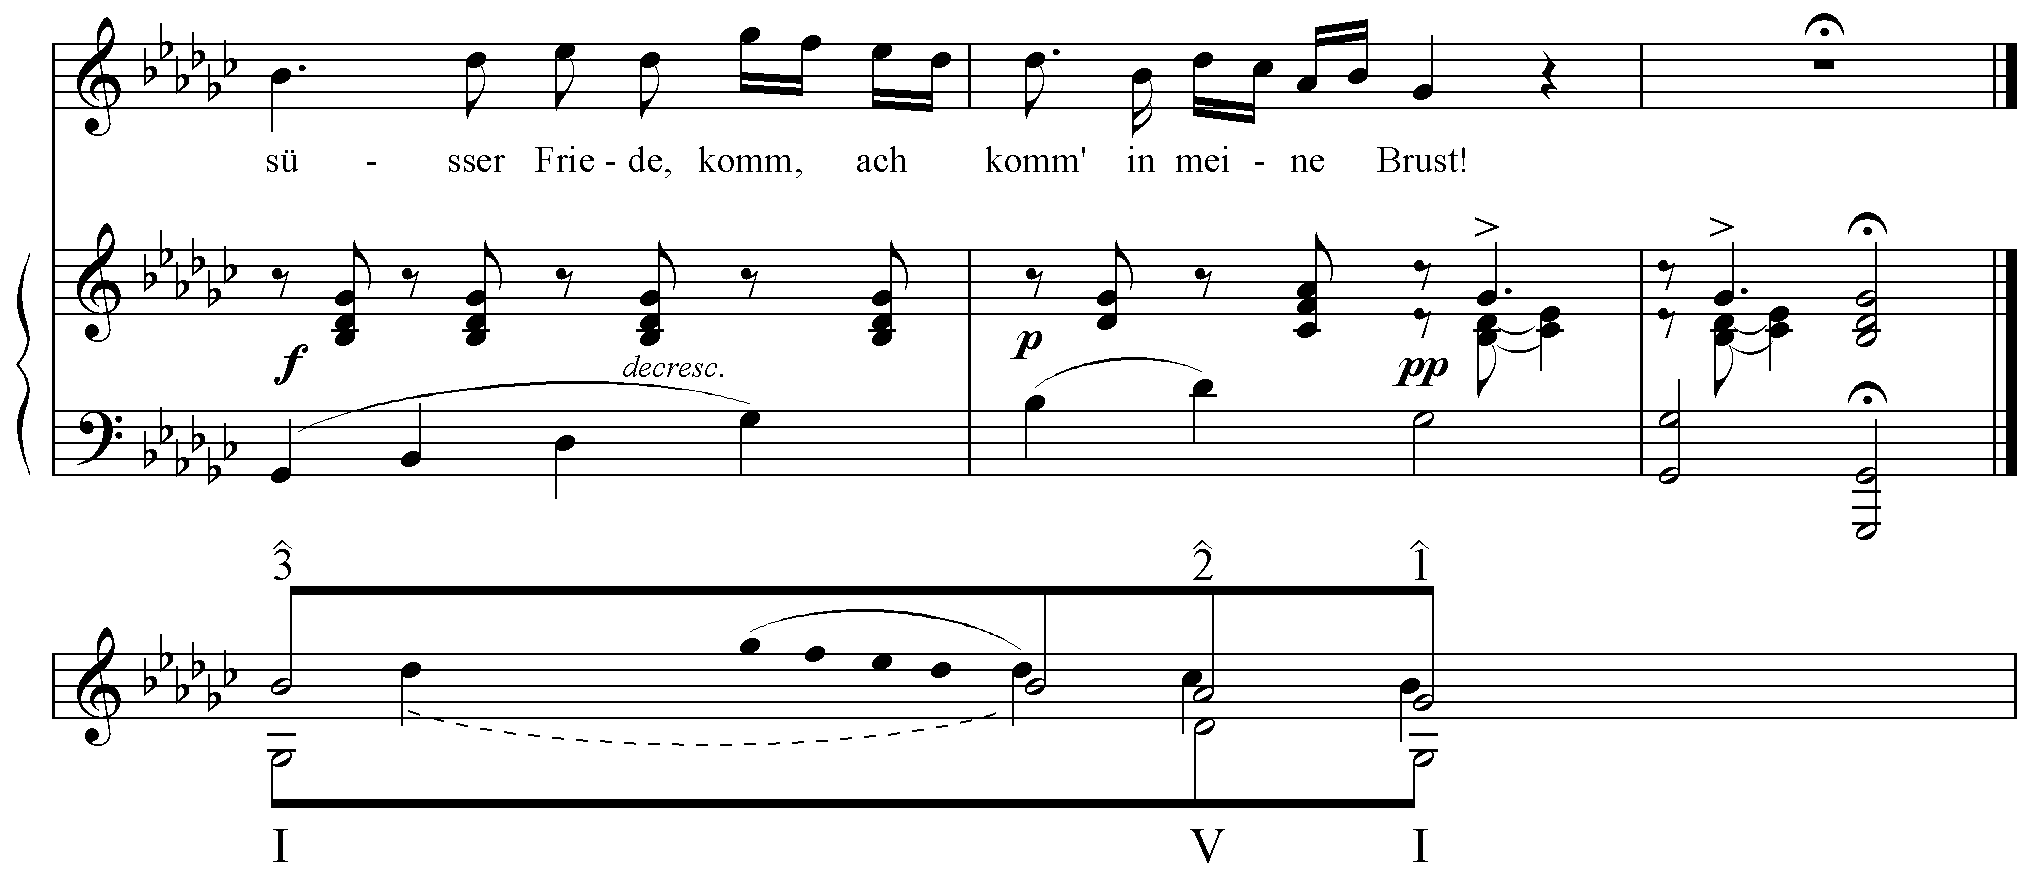
\includegraphics[clip,width=\columnwidth]{figures/schenkerian analysis/SchubertOp4no3.png}% 
\caption[Excerpt of \textit{Wandrers Nachtlied, Op. 4, D. 224} by Franz Schubert.]{\small{Small excerpt of \textit{Wandrers Nachtlied, Op. 4, D. 224} by Franz Schubert. Passage's original score, the schenkerian unfolding of the melody, the chord degrees analysis, and their tonal function.}}
\label{fig:Wandrers Nachtlied, Op. 4, D. 224}
\end{figure}